\subsection{Brute force geometric comparison}

\subsubsection{Segment to Segment Minimum Distance }
The calculation of the distance between segments [8,9] in three dimensions is a geometric calculation that involve getting the closest points by extending the line that they lie on until intersection, if the two lines intersect then the closest point on the two segments is on the boundaries of the segment.
The segment 
$$S1 = [P0, P1]$$
can be formulated as 
$$P(s) = P0+s(P1-P0) = P0+su$$
with a constraint on s, $0<=s<=1$. Similarly, the second segment 
$$S2 = [Q0, Q1]$$
is written as $$Q(t) = Q0+t(Q1-Q0) = Q0+tu$$ with constraint $0<=t<=1$. So, for $sC$ and $tC$ being the closest points on the corresponding extended segments lines L1 and L2, then if  both sC and tC are within the boundaries of the segments then the closest points are also the closest points on the respective segments. 
In the case where sC and tC correspond to points on L1 and L2 outside the range of either segment $S1$ and $S2$, then sC and tC do not also define the closest points on the segments $S1$ and $S2$. So it is necessary to determine points that minimize 
\begin{equation}
w(s,t) = P(s) - Q(t)
\end{equation}
over the ranges of the segments using the corresponding constraints. 
The problem can be formulated into a minimization problem where the equation w is the same as minimizing 
$$|w|^2 = w \cdot w= (P0+su-tv) \cdot (Q0+su-tv)$$

which is a quadratic function of s and t. The relation of $|w|^2$ define a parabolic equation over a (s,t)-plane (See Figure \ref{fig9}) with a minimum at $C = (sC, tC)$, it is strictly growing along the (s,t)-plane with starting point from C. But because segments $S1$ and $S2$ are concerned and not their respective extended lines $L1$ and $L2$, the required minimum region is not C but it is located over a subregion G of the (s,t)-plane. The global minimum at C may lie outside of G, however, in these cases, the minimum always occurs on the boundary of G, and in particular, on the part of G's boundary that is visible to C. That is, there is a line from C to the boundary point which is exterior to G, and it can be said that C can "see" points on this visible boundary of G (See Figure \ref{fig9}).

\begin{figure}[!h]
\centering

\includegraphics[width=0.3\textwidth]{sketches/ss_box} \protect\caption{\label{fig9}(s,t) parameter space with G boundary box C for global minimum}
\end{figure} 

Suppose that we want the minimum distance between two finite segments $S1$ and $S2$, then 
$$G=\{ (s,t) \: \| \: 0 \leq s \leq 1, 0 \leq t \leq 1 \} = [0,1]\times[0,1]$$ 
is a unit square in (s,t) space. The four edges of the square are given by point at $s = 0, s = 1, t = 0, t = 1$. If $C = (sC, tC)$ is outside the G area, then it can "see" at most two edges of G. If $sC < 0$, C can see the $s = 0$ edge, if $sC > 1$, C can see the s = 1 edge, and similarly for tC, so in this way there is an enforcement of the required constraints. When C is not in G, at minimum 1 and at maximum 2 of constraints are active, and they determine which edges of G are candidates for a minimum of $|w| ^2$.
 
For each candidate edge, to compute where the minimum that occurs on that edge, either in its interior or at an endpoint, it is possible to solve for the other unknown parameter since at minimum one is to be found (either t or s). So using the derivative of the $|w^2|$ equation it is always possible to solve for the parameter that is in the interior of G. For example when s = 0, $|w|^2 = ((P0-Q0)-tv) \cdot ((P0-Q0)-tv)$. Taking the derivative with $t$ it possible get a minimum when: $0 = \frac{d}{dt}|w|^2 = -2v \cdot ((P0-Q0)-tv)$.
This gives a minimum on an edge at (0, t0) where $t0 = \frac{(v \cdot (P0-Q0))}{(v \cdot v)}$
If $0 <= t0 < 1$, then this would be the minimum of $|w|^2$ on G, and P(0) and Q(t0) are the two closest points of the two segments. But in the case where t0 is outside G, then either (0,0) or (0,1), would be the minimum along that edge (since $s=0$). Using this method it is possible to perform only a couple of checks to find the minimum of w(s,t) that correspond to the minimum distance between the segments.

\subsubsection{Point to Triangle Minimum Distance}
The other calculation required by the naive approach is to perform the check of point to triangle distance[12, 10, 11]. This test complete the brute force approach since it doesn't leave any  space for cases where triangles are in a configuration where a point - triangle plane distance is the shortest distance in the initial triangle pair minimum distance problem. 

To understand the problem of computing the minimum distance between a point P and a triangle T, it is necessary to understand the parameterised coordinate system of triangles. A triangle can be described by its barycentric coordinates in a way that any point on it can be dependent on two parameters, such that 

$$T(s, t) = B + s \cdot E0 + t \cdot E1$$

where $B = point1$, $E0 = point2-point1$, $E1 = P3 - P1$ for 

$$(s,t) \in D = \{(s,t) : s \in [0,1],t \in [0,1],s + t ≤ 1\}$$ 

The minimum distance is computed by determining the values $(s, t) \in D$ in the squared-distance equation $Q(s, t) = |T(s, t) - P|^2$ where $T(s,t)$ correspond to a point on the triangle closest to P. The function is quadratic and can be written as: 
$$Q(s,t)=as^2 +2bst+ct^2 +2ds+2et+f$$

where $a = E0 \cdot E0$, $b = E0 \cdot E1$, $c = E1 \cdot E1$, $d = E0 \cdot (B - P)$, $e = E1 \cdot (B - P)$, and $f = (B - P) \cdot (B - P)$.

Quadratics are classified by the sign of $ac - b^2$ so for function Q, $ac - b2$ = $(E0 \cdot E0)(E1 \cdot E1) - (E0 \cdot E1)^2$ =$|E0 \cdot E1|^2 >0$. The positivity is based on the assumption that the two edges E0, E1 are linearly independent, so their cross product is a nonzero vector. Q is a continuously differentiable and the minimum occurs at an interior point of D where the gradient $Q = 2(as + bt + d, bs + ct + e) = (0, 0)$ or at a point on the boundary of D. The gradient of Q is zero only when 
$$s = (be - cd)/(ac - b^2)$$ and 
$$t = (bd - ae)/(ac - b^2).$$ 
If $(s,t) \in D$, then minimum of Q is found. For example considering that region 0 (See Figure \ref{fig10}) is the domain of Q, so $(s, t) \in D$. If (s, t) is in region 0, then the point on the triangle closest to P is interior to the triangle, not on its edge.

\begin{figure}[!h]
\centering
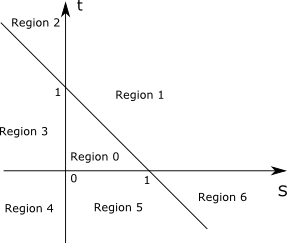
\includegraphics[width=0.4\textwidth]{sketches/pt_regions} \protect\caption{\label{fig10} Regions based on the (s,t) parameters plane}
\end{figure} 

On the other hand if the minimum is not in D then it should be should be on the boundary of the triangle and using the correct active constraints to restrict the solution using the region methodology. So if (s, t) is in region one then the elliptic level curves of Q are those curves in the s,t plane for which Q is constant. 

At the point where Q = (0,0), the level curve degenerates to a single point (s, t). The global minimum of Q occurs there ($V_{min}$). As the level values V increase from $V_{min}$, the corresponding levels are growing away from $(s,t)$. There is a smallest level value V0 for which the corresponding ellipse is tangent to the triangle domain $D$ edge $s+t = 1$ at a value $s = s0 \in [0,1], \: t0 = 1 - s0$. So for any level values $V < V0$, the corresponding ellipses do not intersect $D$. However for any portion of $D$ that intersect elliptic levels V must be $V > V0$. Therefore in this case point $(s0, t0)$ provides the minimum distance between P and the triangle where $t0$ is known $t0 = 1 - s0$ and $s0$ is the only unknown to be solved since the problem is decreased by one dimension. Moreover, when minimization is happening at $\nabla Q(s, 1 − s) = 0$ then there are three cases where $s > 1$ and $s$ has to be restricted to $s=1$ and the minimum occurs at $\nabla Q(1, 0)$ because of the barymetric triangle constraints, similarly if $s < 0$ then minimum occurs when $\nabla Q(0,1)$ or lastly $s \in [0,1]$ and has to be solved for a minimum at $\nabla Q(s,1-s)$.

Similarly the same technique for determining whether the minimum occurs at the endpoints or at the interior interval of the corresponding constraints, is performed for region three and region five (Figure \ref{fig10}). In the case where (s, t) occur in region three then the minimum has to occur at (0, t0) following the process like in region one where $t0 \in [0, 1]$. If $(s, t)$ is located in region five (Figure \ref{fig10}), then the minimum occurs at $(s0, 0)$ where $s0 \in [0, 1]$.  

When $(s, t)$ is located inside region two, there are three possibilities for the elliptic level curve that contact or intersect the boundaries of $D - region0$ area, the contact of the levels with the triangular region may occur in: 
\begin{enumerate}
\item edge where $s + t = 1$ 
\item edge where $s = 0$
\item at point where $t = 0$ and $s = 1$.
\end{enumerate}

That is because although the global minimum occurs in region two, there is a level curve of Q that contact the $D$ but the contact point and the region inside the level curve does not overlap. At these occurrences then the negative of the contacting level curve of Q cannot point inside $D$. For example for region two could be the direction of $-\nabla Q(0,1), -\nabla Q(s,1-t) and -\nabla Q(0,t),$ which points towards the inside of the level curve instead of inside $D$. 

In order to determine which of the three cases occur, it is possible to check which areas are negative so in a way it is possible to eliminate the cases where the contact doesn't occur and where it does. So if $\nabla Q = (Qs, Qt)$ and $Qs$ and $Qt$ are the partial derivatives of Q, it should be the case where $(0, -1) \cdot \nabla Q(0, 1)$ and $(1, -1) \cdot \nabla Q(0, 1)$ are not both  negative. The two vectors $(0, −1)$ and $(1, −1)$ are directions that correspond to the edges $s = 0$ and $s + t = 1$, respectively. The choice of edge $s+t = 1$ or $s = 0$ can be made based on the signs of $(0,-1) \cdot \nabla Q(0,1)$ and $(1, -1) \cdot \nabla Q(0, 1)$. Similarly as for region three, the same calculation technique is used for the regions four and six. 

\clearpage

\begin{algorithm}
 \caption{Brute-force distance calculation.} \label{algorithm:bf}
 \begin{algorithmic}[1]
	\Function{BF}{A, B, C, D, E, F}
	
		\State $T1=[A;B;C;];$
		
		\State $T2=[D;E;F;];$

		\State $list[0]= pt(T2, T1[0]);$

		\State $list[1]= pt(T2, T1[1]);$

		\State $list[2]= pt(T2, T1[2]);$

		\State $list[3]= pt(T1, T2[0]);$

		\State $list[4]= pt(T1, T2[1]);$

		\State $list[5]= pt(T1, T2[2]);$

		\State $ptmin = min(list);$

		\State $list[0]=segseg(T1[0],T1[1],T2(0],T2[1]);$

		\State $list[1]=segseg(T1[0],T1[1],T2[1],T2(2]);$

		\State $list[2]=segseg(T1[0],T1[1],T2[2],T2(0]);$

		\State $list[3]=segseg(T1[1],T1[2],T2[0],T2(1]);$

		\State $list[4]=segseg(T1[1],T1[2],T2[1],T2(2]);$

		\State $list[5]=segseg(T1[1],T1[2],T2[2],T2(0]);$

		\State $list[6]=segseg(T1[2],T1[0],T2[0],T2(1]);$

		\State $list[7]=segseg(T1[2],T1[0],T2[1],T2(2]);$

		\State $list[8]=segseg(T1[2],T1[0],T2[2],T2(0]);$

		\State $ssmin = min(list);$

		\State $min = min(ssmin, ptmin);$

		\State $P = min.p; Q = min.q;$
	\EndFunction
 \end{algorithmic}
\end{algorithm} 


\begin{algorithm}
 \caption{Point to triangle distance algorithm.} \label{algorithm:bf}
 \begin{algorithmic}[1]
	\Function{pt}{T, Point}
		
		%function to evaluate Q(s,t) of triangle T 		
		
		\If{PointProjection in Region 0}
		
			\State {evaluate value of Q}
		
		\EndIf		
		
		\If {PointProjection in Region 1}
		
			\State {determine (s,t) parametric space values}
		
		\EndIf
			
		\If {PointProjection in Region 2}

			\State {determine (s,t) parametric space values}

		\EndIf			
		
		\If {PointProjection in Region 3}
		
			\State {determine (s,t) parametric space values}

		\EndIf
						
		\If {PointProjection in Region 4}
		
			\State {determine (s,t) parametric space values}
		
		\EndIf
				
		\If {PointProjection in Region 5}		

			\State {determine (s,t) parametric space values}

		\EndIf
				
		\If {PointProjection in Region 6}	

			\State {determine (s,t) parametric space values}
			
		\EndIf		
		
		\Return $Q point on triangle$
	\EndFunction
 \end{algorithmic}
\end{algorithm} 

\begin{algorithm}
 \caption{Segment to segment distance algorithm.} \label{algorithm:bf}
 \begin{algorithmic}[1]
	\Function{pt}{segment1, segment2}
		
		%function to evaluate (s,t) of seg1, seg2
		\If {segment1 and segment2 are parallel}		
		
			\Return {any point P on segment1 and any point Q on segment2}
		
		\Else 
			
			\State {Get the closest points sC and tC on the infinite lines L1, L2}
			
			\If {sC < 0, the s = 0 edge is visible}
				
				\State {s = 0}
				
			\EndIf
				
			\If {sC > 0, the s = 1 edge is visible}

				\State {s = 1}			
				
			\EndIf
				
			\If {tC < 0, the t = 0 edge is visible}

				\State {t = 0}

			\EndIf
								
			\If {tC > 0, the t = 1 edge is visible}

				\State { t = 1}

			\EndIf							
		\EndIf
		
		\Return {P, Q points on two segments}
		
	\EndFunction
 \end{algorithmic}
\end{algorithm} 

%
% How does the algorithm work. Robustness
%
Our default brute force approach implementation runs per triangle pair through all possible distance
configurations (Algorithm \ref{algorithm:bf}).
First, we run through all six involved vertices and compute the distance to the
other triangle.
Second, we determine the distances between each line segment-to-line segment combination.
This yields 9+6=15 comparisons in total.
The minimum distance results from a minimum over all computed distances.
It is a robust approach, it always yields the correct answer.


%
% Speed, character
%
The algorithm is \ldots 

A fusion of multiple steps is not possible since all parametric/geometric scenarios have to be evaluated separately and naively. As shown the algorithm in Figure (x) the geometric checks and the brute force character of the algorithm does not allow computational fusion of execution branching. 



